\chapter{Test case}
\textbf{TODO}
%TODO SI PUO' eliminare l'agente postman?
%TODO trasformare l'agente deposito in spazio di tuple, la consegna fatta tramite 'write'

\section{Descrizione problema}
Il quesito che è stato preso in esame per presentare le funzionalità del progetto sviluppato è noto come `Goldminers' ed è stato definito da Jomi H\"ubner e Rafael Bordini.

\medskip
\fbox{\parbox[t][][t]{1\textwidth}{
In questo scenario un gruppo di agenti minatori deve recuperare pepite d'oro da miniere sparse nell'ambiente e riportarle in un deposito.
}}
\medskip

Il quesito è stato quindi applicato al progetto realizzato in questo lavoro di tesi e sono stati delineati i comportamenti dei ruoli (minatore, miniera, deposito) all'interno della scena: ognuno di essi sarà una specializzazione dell'agente. All'interno di ogni nodo sarà contenuto solo un agente, oltre a quello per il movimento che è `fissato' nel nodo, per via dell'implementazione dell'interprete.
\\
Nella scena gli agenti sono posizionati casualmente all'interno di aree delimitate da cerchi, i quali sono posizionati nell'ambiente secondo le direttive della configurazione. Per ogni tipologia di ruolo è definita l'area del cerchio nel quale sono posizionati gli agenti.
\\
Qui di seguito è descritto come il problema sarà implementato all'interno dell'interprete realizzato.

I minatori conoscono la posizione del deposito: il loro compito è quello di recuperare le pepite e consegnarle al deposito.
Le miniere sono contenitori di risorse, le pepite, che sono estratte dai minatori. Il numero di pepite contenute all'interno di ogni miniera è casuale.

Quando inizia la simulazione i minatori si muovono nell'ambiente alla ricerca di una miniera. Lo spostamento dei nodi viene comandato dall'agente minatore secondo la distribuzione di Levy.
Se il minatore incontra una miniera prova a prelevare una pepita e una volta recuperata la risorsa avvia lo spostamento verso il deposito per recapitare la pepita. Dopo la consegna il minatore riparte verso la miniera da cui ha estratto la risorsa per continuare ad estrarre fino ad estinguerla.
Quando il minatore esaurisce la miniera torna allo stato iniziale, ovvero muovendosi nell'ambiente alla ricerca di nuove miniere da cui estrarre pepite.


\subsection{Tematizzazione della simulazione}
Alchemist nella finestra della simulazione permette di definire degli effetti da applicare ai nodi della simulazione per tematizzarli. La finestra attraverso la quale è possibile definire lo stile è mostrata in Figura \ref{fig:tematizzazioneSimulazione}.

%crea l'ambiente figura;
\begin{figure}[h] % [h] sta per here, cioè la figura va qui
\begin{center} % centra nel mezzo della pagina la figura
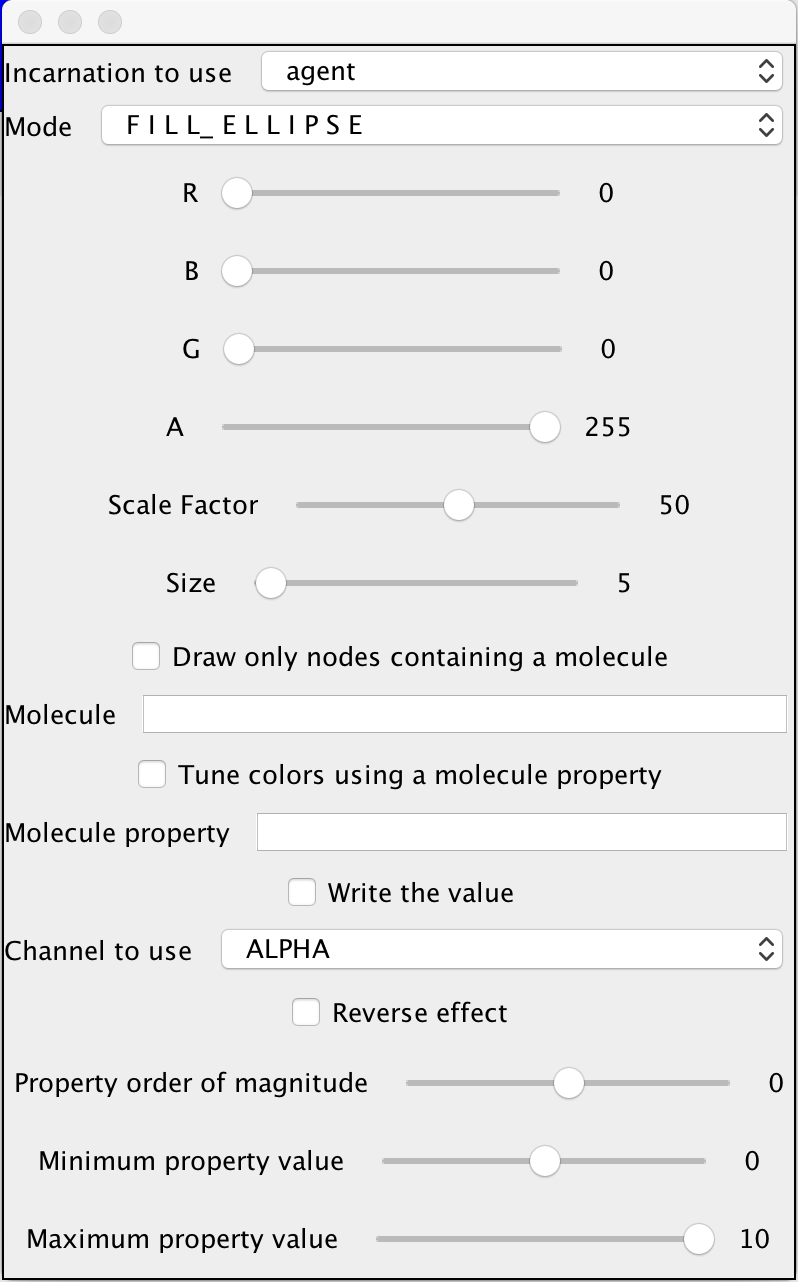
\includegraphics[width=6cm]{images/tematizzazioneSimulazione.png} % inserisce una figura larga 12.5cm
% inserisce la legenda ed etichetta la figura con \label{fig:prima}
\caption[Tematizzazione della simulazione]{Tematizzazione della simulazione} \label{fig:tematizzazioneSimulazione}
\end{center}
\end{figure} 

Dall'immagine si può osservare che l'effetto può essere composto da molteplici fattori.
Per quanto riguarda la tematizzazione scelta per questa simulazione sono stati utilizzati i controlli presenti nella prima metà della finestra.
\newline

Sono state definite delle stringhe identificative per le molecole e che si riferiscono univocamente i vari ruoli nella scena: minatore (miner), miniera (goldmine), deposito (deposit), pepita (nugget).
Per stringa è stato creato un relativo stile definito da un colore (tramite il modello RGBA), un fattore di scala e una dimensione per rappresentare il nodo.
\\
L'associazione tra ogni effetto e la rispettiva molecola viene realizzato spuntando la casella di controllo relativa a `Draw only nodes containing a molecule' ed inserendo nella casella di testo sottostante la stringa identificativa della molecola che si vuole abbinare.
\newline

Nell'implementazione dell'interprete sono opportunamente create le molecole utilizzando la classe SimpleMolecule passando come parametro l'identificativo le stringhe descritte poco sopra. Gli oggetti istanziati sono poi inseriti all'interno del nodo.

Una volta creato lo stile desiderato è possibile salvarlo (viene generato un file con estensione .aes) in modo da poterlo riutilizzare.
All'avvio di una simulazione di default non è presente nessuna tematizzazione però è possibile caricare un file salvato in precedenza.
La tematizzazione non è necessaria al fine dell'esecuzione della simulazione ma è molto utile per poter comprendere al meglio il comportamento degli agenti nell'avanzamento della simulazione.


\section{Implementazione agenti}
In questa sezione è descritto come sono state create le teorie e le classi degli agenti che sono stati implementati per la realizzazione dello scenario di test.

\textbf{TODO - completare}


\subsection{Miniera}
La miniera è un'entità che è posizionata in modo casuale all'interno dell'ambiente, che mantiene la sua posizione nel tempo e che contiene delle risorse.
Data questa descrizione la sua realizzazione è stata subito associata agli spazi di tuple. Si è quindi implementata la classe Goldmine estendendo la classe AbstractSpatialTuple.

\subsubsection{Teoria tuProlog miniera}

\medskip
\begin{lstlisting}[firstnumber=1,label={lst:Goldmine},caption={Teoria miniera}]
init :-
    agent <- generateNextRandom returns RAND,
    NUGGETS is RAND * 1.0,
    loadNuggets(NUGGETS).

loadNuggets(NUGGETS) :-
    NUGGETS > 0,
    assertz(nugget),
    N is NUGGETS - 1,
    loadNuggets(N).

loadNuggets(NUGGETS) :-
    NUGGETS < 0,
    agent <- setConcentration.
\end{lstlisting}


\subsubsection{Implementazione classe Goldmine}



\subsection{Minatore}

\subsubsection{Teoria tuProlog minatore}

\subsubsection{Implementazione classe Miner}




\subsection{Deposito ???}





\section{Configurazione della simulazione}
Per definire la simulazione si deve scrivere un'opportuna configurazione nella quale sono descritti, attraverso le keyword, quali oggetti utilizzare nella simulazione in relazione al modello creato. Nel Codice sorgente \ref{lst:GoldminersSimulation} sono mostrate e descritte in dettaglio le varie parti che compongono la configurazione e che sono state precedentemente spiegate nella sezione \ref{sctn:ScrivereUnaSimulazione}.

\medskip
\begin{lstlisting}[firstnumber=1,label={lst:GoldminersSimulation},caption={Configurazione simulazione Goldminers}]
incarnation: agent

network-model:
  type: ConnectWithinDistance
  parameters: [2]

displacements:
  - in: {type: Circle, parameters: [2,2,2,0.2]}
    programs:
      -
        - time-distribution: 9
          program: "miner"

  - in: {type: Circle, parameters: [1,2,2,0.2]}
    programs:
      -
        - time-distribution: 9
          program: "deposit"

  - in: {type: Circle, parameters: [1,2,2,0.2]}
    programs:
      -
        - time-distribution: 9
          program: "postman"

  - in: {type: Circle, parameters: [10,2,2,5]}
    programs:
      -
        - time-distribution: 9
          program: "goldmine"
\end{lstlisting}

La prima cosa che si può notare nella configurazione è la specifica dell'incarnazione utilizzata `agent', ovvero quella definita per questo progetto.
\newline

Il secondo parametro impostato in configurazione è il `network-model', il parametro che definisce la `linking-rule', che descrive in che modo ogni nodo presente all'interno dell'ambiente è collegato con gli altri. Attraverso questa regola cambia il numero di nodi presenti nel vicinato di ogni nodo. Nel caso specifico, è stato scelto di utilizzare una classe che utilizza la relazione di distanza per collegare i vari nodi ed alla quale è stato passato come parametro il valore 2; per ogni nodo, sono considerati suoi vicini tutti i nodi che ad ogni istante della simulazione siano posizionati all'interno di un cerchio di dimensione 2 il cui centro è il nodo stesso.
\newline

Il terzo ed ultimo parametro è `displacements' che definisce una lista con la disposizione dei nodi ed il loro contenuto.
\\
La lista si compone di due keyword: $in$ e $programs$. La prima richiede un oggetto che definisce il tipo della geometria e i parametri per costruirla, mentre la seconda utilizza un'ulteriore lista all'interno della quale sono definite le reazioni associate ad ogni nodo.

Per tutti i ruoli della scena è stato utilizzato il cerchio come geometria per posizionare i nodi, passando per ognuno dimensioni e quantità di nodi differenti.
\\
Attraverso la keyword $program$ si definiscono le reazioni che saranno inserite nei nodi: come si può notare dalla configurazione, per ogni nodo è stata definita una sola reazione.
Per definire una reazione sono stati utilizzati una distribuzione temporale ed una stringa; quest'ultima sarà poi utilizzata durante la creazione di istanze della classe AgentReaction e con la quale verrà istanziata all'interno della reazione la classe dell'agente relativa.
\\
Come parametro della distribuzione temporale è stato scelto 9: questo valore ha consentito, anche in base al valore di distribuzione temporale associato all'azione di spostamento posizionata in maniera intrinseca nel nodo, di avere un comportamento che è sembrato molto fluido.






------sotto solo per copia di alcuni pezzi





\subsection{Implementazione teoria agenti}
Per realizzare la simulazione di questo esempio si è partiti dalla definizione delle teorie dei vari ruoli all'interno della scena. Qui di seguito sono descritte ed analizzate le teorie degli agenti definiscono i comportamenti degli agenti durante l'esecuzione della simulazione.
\\
La parte non descritta in questa sezione è quella relativa alle classi dell'interprete.


\subsubsection{Miniera - Goldmine}
Per la realizzazione della miniera si è subito pensato ad una specializzazione della classe AbstractSpatialTuple che permettesse di recuperare le risorse contenute al suo interno tramite l'utilizzo delle primitive spaziali, più precisamente della primitiva $out$ definita nel linguaggio realizzato tramite $takeTuple(TT)$. La teoria di questo agente è poco complessa poichè definisce solamente il caricamento di un numero casuale di risorse (ovvero le tuple) all'interno dello spazio di tuple.

\medskip
\begin{lstlisting}[firstnumber=1,label={lst:Goldmine},caption={Teoria miniera}]
init :-
    agent <- generateNextRandom returns RAND,
    NUGGETS is RAND * 1.0,
    loadNuggets(NUGGETS).

loadNuggets(NUGGETS) :-
    NUGGETS > 0,
    assertz(nugget),
    N is NUGGETS - 1,
    loadNuggets(N).

loadNuggets(NUGGETS) :-
    NUGGETS < 0,
    agent <- setConcentration.
\end{lstlisting}
Nel corpo della regola $init$ viene inizialmente recuperato un numero random, attraverso l'invocazione del metodo $generateNextRandom()$ definito nell'agente, che rappresenta le pepite da posizionare all'interno della miniera. Il caricamento delle risorse viene fatto tramite l'invocazione della regola $loadNuggets(NUGGETS)$ con la quale sono inseriti i fatti nello spazio di tuple: se le risorse sono state tutte caricate viene invocato il metodo $setConcentration()$, anch'esso definito nell'agente, che viene utilizzato per tematizzare graficamente lo spazio di tuple nella simulazione.

\subsubsection{Deposito - Deposit}
TODO

\subsubsection{Minatore - Miner}
TODO

\subsection{Implementazione classi agenti}

\subsubsection{Miniera - Goldmine}
TODO

\subsubsection{Deposito - Deposit}
TODO

\subsubsection{Minatore - Miner}
TODO









\section{Vantaggi approccio scelto}
